\section{Case Study: Expert Analysis of Medical Outcome}
\label{sec:case_study}

The proposed workflow described above stem from a one year collaboration with a machine learning expert and a medical doctor from the \textit{NYU Langone Medical Center}, both co-authors of this paper. The medical machine learning team at the medical center works in tight collaboration with doctors and hospital management to derive novel methods to automate medical procedures, provide diagnostics support, improve efficiency and gain novel insights on medical procedures and processes.

\noindent \textbf{Domain Problem Description.}
Our collaboration focused on the analysis and improvement of models built to optimize processing times in the emergency department of the hospital. The crucial decision here is whether a patient coming to the emergency room will end up being admitted to the hospital or sent home. In the case of a patient being admitted to the hospital, a bed has to be prepared for the patient which results in a 2-hour waiting period where the patient occupies a bed in the emergency room preventing other patients from being processed. If the waiting time can be reduced by knowing early if a given patient will be admitted, the throughput of the emergency room can be increased.

\begin{figure}
\centering
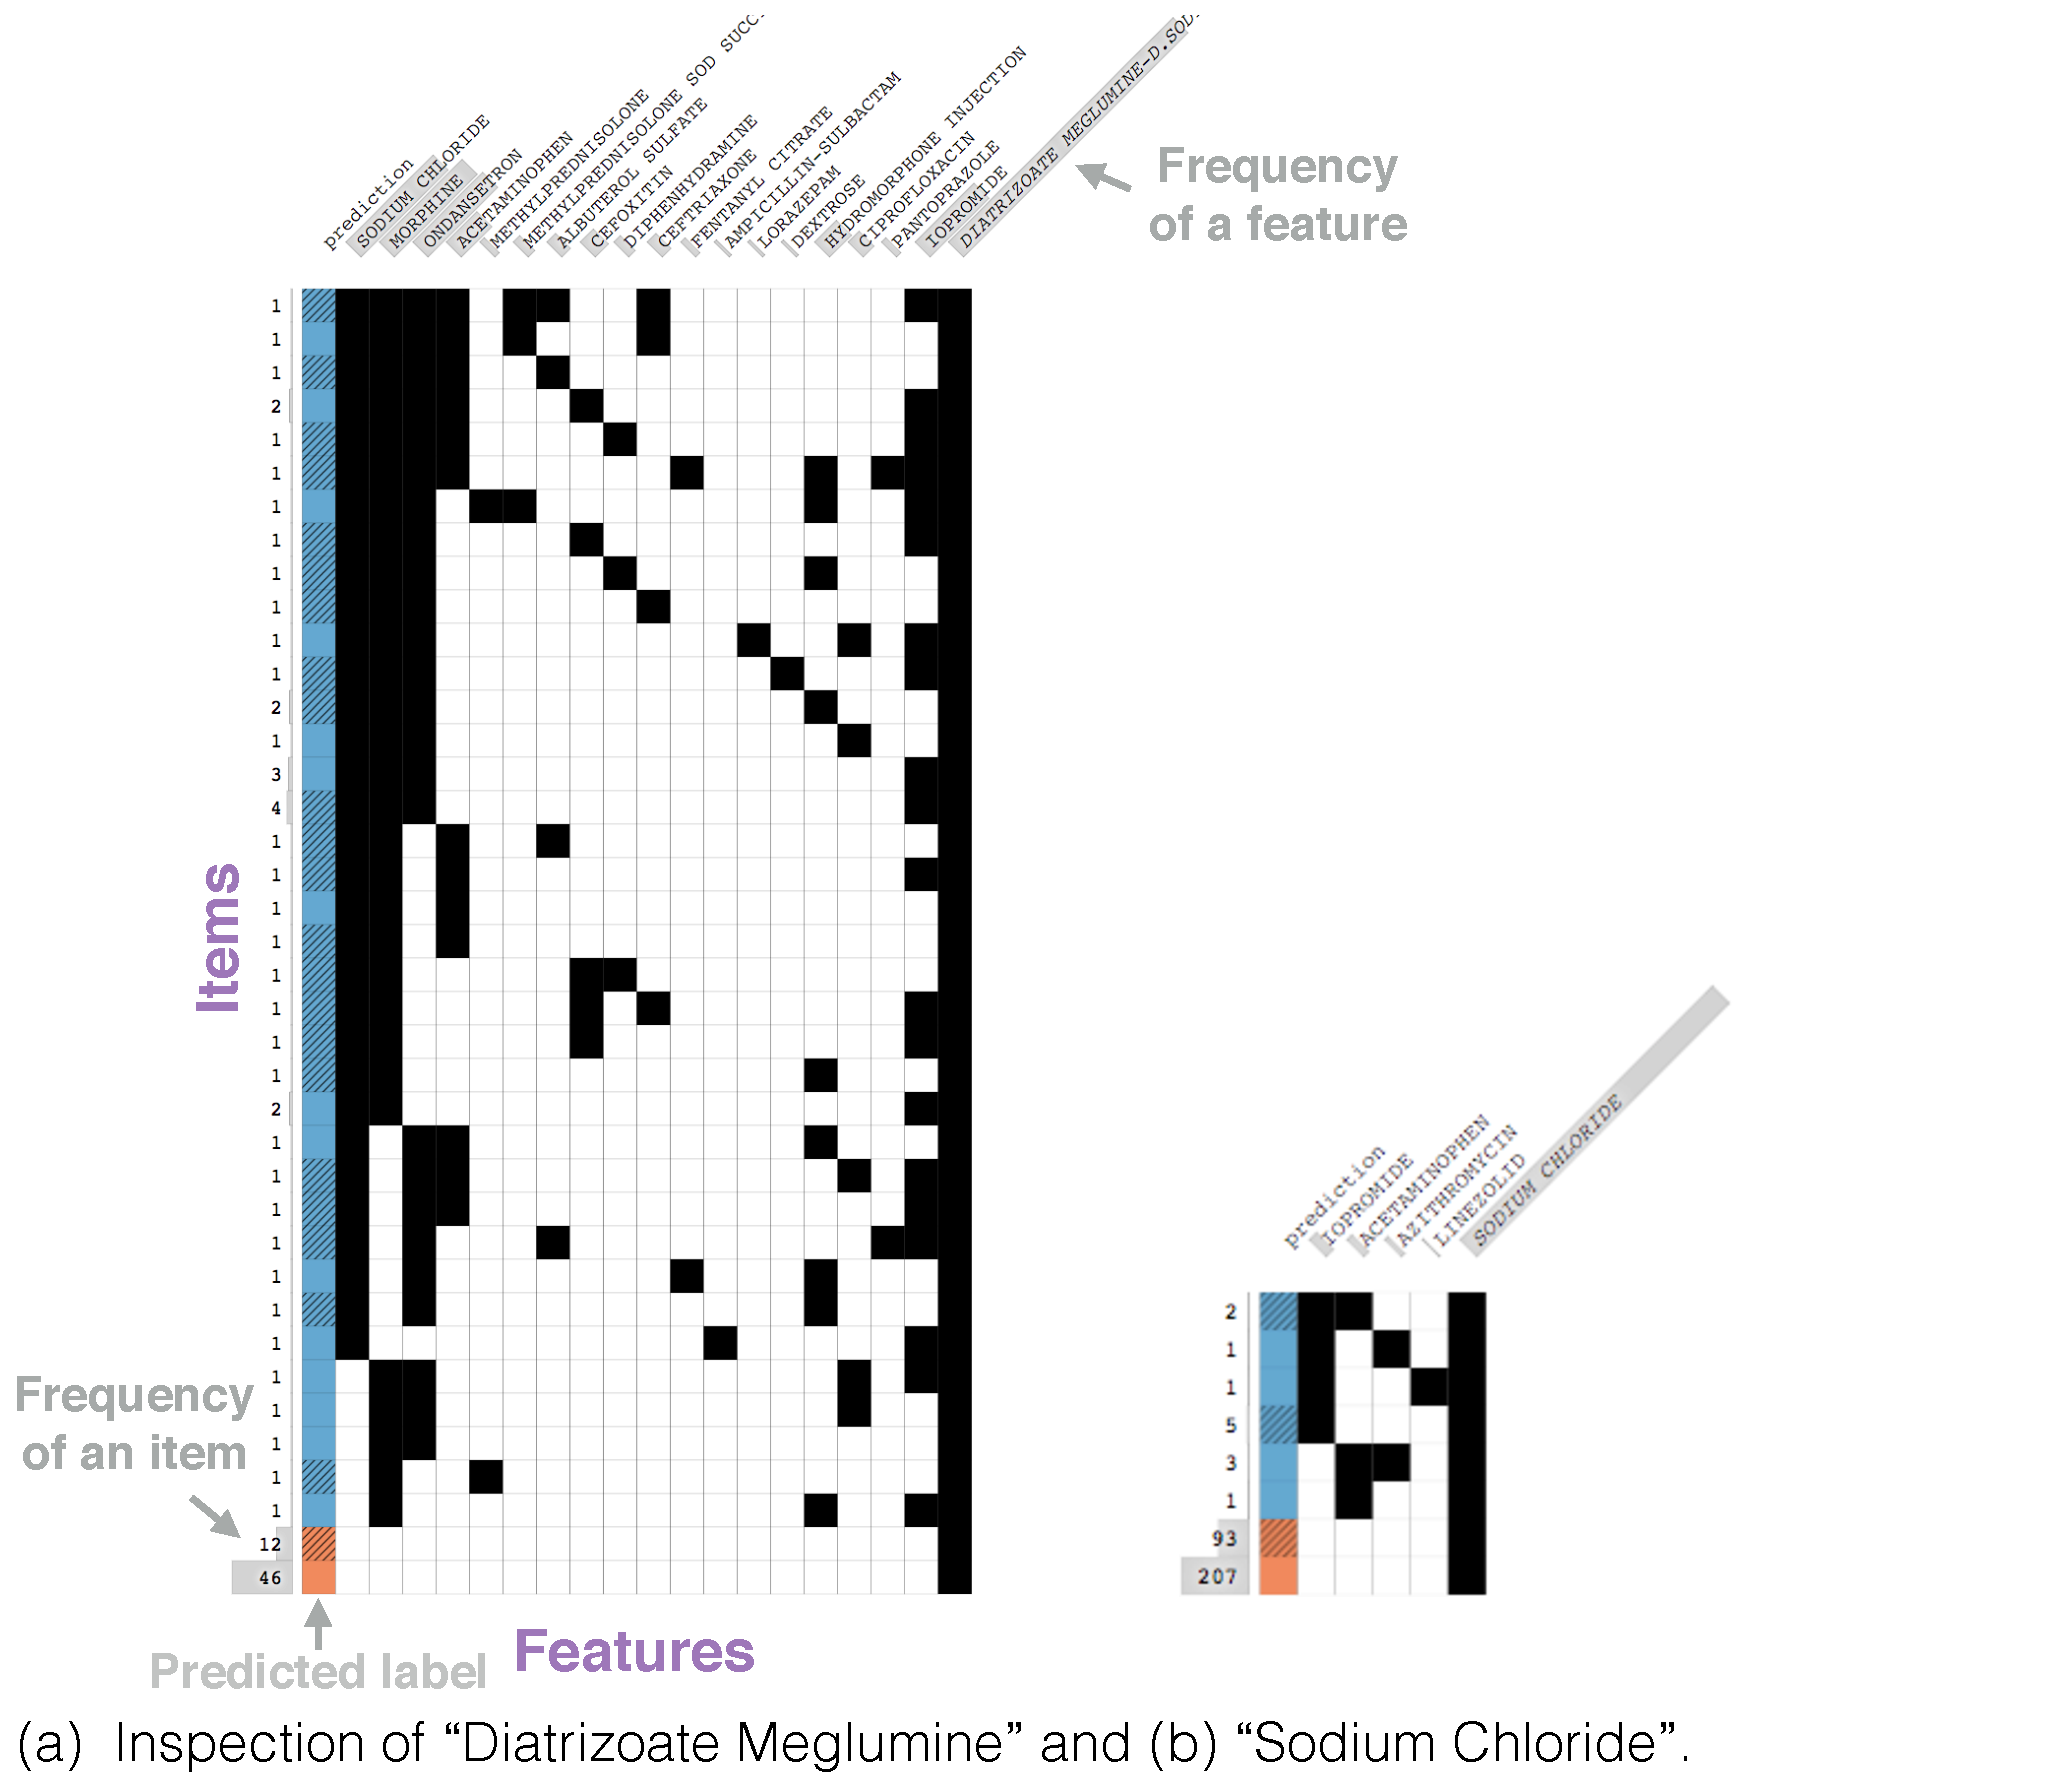
\includegraphics[width=\linewidth]{explainer/inspect1}
% \begin{subfigure}[b]{0.7\linewidth}
%     \centering
%     \includegraphics[width=\linewidth]{fig/inspect}
%     \caption{~Inspection of ``Diatrizoate Meglumine"}
%     \label{figs:inspect}
% \end{subfigure}
% \hspace{-3em}
% \begin{subfigure}[b]{0.35\linewidth}
%     \centering
%     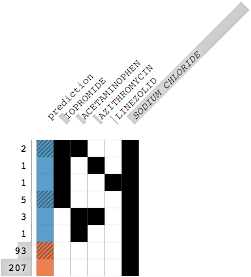
\includegraphics[width=1.03\linewidth]{fig/sodchl} % warning here is necessary
%     \caption{~and ``Sodium Chloride".}
%     \label{figs:sodchl}
% \end{subfigure}
\caption[The \tabC.]{
The \textbf{\tabC} showing a matrix of data items as rows and features as columns for the explanations \emph{Diatrizoate Meglumine} and \emph{Sodium Chloride} in the initial data set of the case study (Section~\ref{sec:case_study}).
Rows group identical instances together and show the count on the left side.
Features are sorted by ``relative feature importance" showing from left to right how labels can be separated.
% \aritra{This figure needs annotations: Items, Features, Predicted Label, and what the bars mean}
% \joschi{too much info here}
}
\label{figs:inspect_all}
\end{figure}

The idea to reduce this wait time is to use predictive modeling at the earliest time possible so that an admitted patient can be moved sooner. The amount of data available to make this decision however is very limited. When first presented with a patient the emergency doctor orders medication for treating, stabilizing, or preparing the patient for procedures or tests and eventually will conclude a diagnosis and decide whether the patient is in need of admission.

As medication is the earliest recorded indicator of the admission result and also is recorded before lengthy procedures or tests it is the most promising candidate for a predictive model. The main machine learning task is therefore to verify whether a viable model can be built by using exclusively the limited information available.
% 0:20:00;00

Other work has been done in this regard, however, using input features that are not readily available (\eg, information from medical notes that are written after the fact) or are hospital specific (\eg, mode of arrival, triage score) \cite{pmid21705374,pmid24421344,pmid24509606}.

%When patients enter the emergency room it is hard to predict whether they will be ultimately admitted or sent back home after treatment (this is relevant information the hospital needs to optimize the process). The main machine learning task addressed by the project is to verify if it is possible to predict whether a patient will be admitted or not by looking exclusively at the set of drugs the patient has received. This is the only information that can be collected reliably and automatically within the first two hours after a patient enters the hospital and therefore the only information that can be used to build the machine learning model.

\begin{figure}
\centering
\begin{subfigure}[b]{\linewidth}
    \hfill
    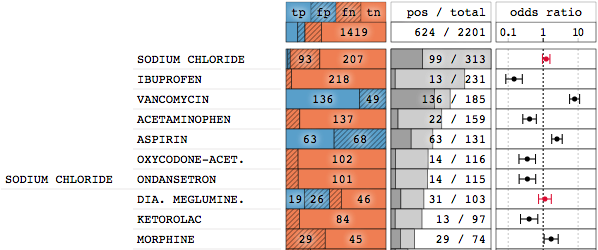
\includegraphics[height=7em]{explainer/expl_10_size}
    \caption{~Ordered by ``total" size showing the most common explanations.}
    \label{figs:expl_10_size}
\end{subfigure}
\\
\begin{subfigure}[b]{\linewidth}
    \hfill
    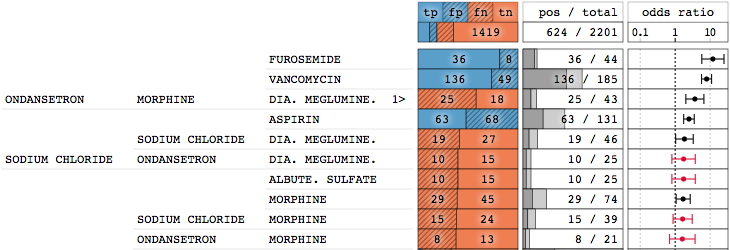
\includegraphics[height=7em]{explainer/expl_10_or_pos}
    \caption{~Ordered by ``odds ratio" showing significantly positive explanations.}
    \label{figs:expl_10_or_pos}
\end{subfigure}%
\\
\begin{subfigure}[b]{\linewidth}
    \hfill
    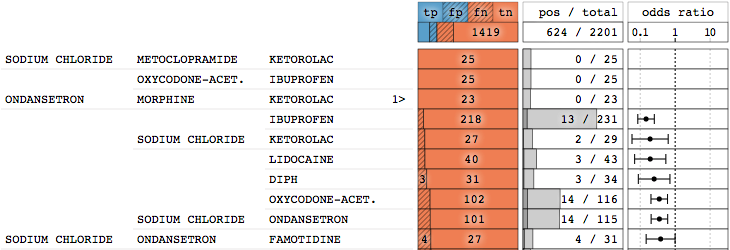
\includegraphics[height=7em]{explainer/expl_10_or_neg}
    \caption{~Ordered by reverse ``odds ratio" showing significantly negative explanations.}
    \label{figs:expl_10_or_neg}
\end{subfigure}%
\\
\begin{subfigure}[b]{\linewidth}
    \hfill
    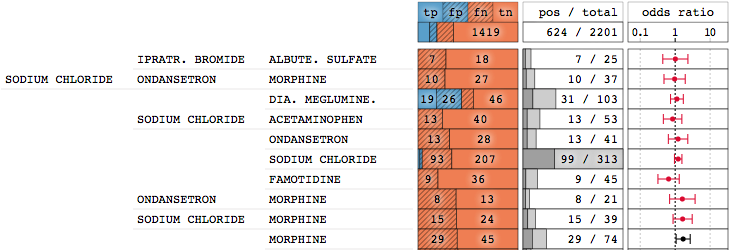
\includegraphics[height=7em]{explainer/expl_new_uncertain}
    \caption{~Ordered by ``uncertainty" showing item subsets whose predictions are not significant.}
    \label{figs:expl_10_uncertain}
\end{subfigure}
\caption{
Showing different orders in the \textbf{\tabB} for addressing the goals (G2 \& G3) in the case study (Section~\ref{sec:case_study}). The initial dataset is filtered for explanations with $> 20$ data items.
% The \textbf{\tabB} showing the initial case study dataset (see Section~\ref{sec:case_study}) filtered for explanations with $> 20$ data items.
}
\end{figure}

During our collaboration the team of visualization experts met with the medical team regularly to understand the problem and the data, and to develop collaboratively visual analytics solutions for model diagnostics and interpretation. The workflow we described in the paper resulted from numerous iterations over the methods used to derive information from the model and the methods used to enable their interactive visual exploration.

In this section, we describe one particular example that showcases the capabilities of the proposed method and provides insights on how it is able to support diagnostic analysis of complex machine learning model used in a relevant real-world scenario. In the following, the term ``we" is used to refer to the team of visual analytic experts, a machine learning expert, and a medical doctor, who collaboratively worked on the usage scenarios described below.

\noindent \textbf{Selecting Initial Data and Model (G1).}
% \joschi{In the following the term ``we" is used to refer to the visual analytics experts, machine learning expert, or medical doctor, given by the context.}
We initially gathered a dataset of 5980 patients ($28\%$ admitted) with binary vectors indicating medications given to the patient. Those patients were randomly split into a training (1196 patients with $30\%$ admitted) and test (4784 patients with $27\%$ admitted) dataset. We then computed several models and tweaked them using mostly the \tabA and model specific approaches.
This initial dataset contains 398 unique medications.
The table below shows a summary of the models we trained and their performance.
%were developed over several months with a regular back-and-forth with domain experts.
% Following, we describe how we were able to use our workflow and user interface to improve quality of and trust in a particular machine learning task.
% Additionally, we show that we can detect certain classes of modeling errors by constructing artificial datasets with known biased behaviors.

%Our main motive for the proposed workflow and user interface is based around a medical case study of using predictive modeling to optimize processing times in the emergency department of hospitals.

%Algorithms like a Random Forest~\cite{Breiman:2001:RF:570181.570182} risk overfitting. This is indicated when the AUC on the training dataset is much higher than the AUC on the test dataset.

%Furthermore, overfitting can be seen with explanations as well when sorting rows in the \tabB by descending explanation length. Models that single out specific data items do not generalize very well. This can be seen when many long explanations ($> 5$) exist that only capture very few data items ($< 5$). How problems like overfitting can be mitigated depends on the classification algorithm and its model parameters.

%In the case of Random Forests increasing the number of trees and decreasing their allowed height helps.

%From an initial train/test AUC of 0.95/0.74 we were able to improve the model to a train/test AUC of 0.88 / 0.79. For other models different hyper-parameters can be adjusted.

\begin{center}
\begin{tabular}{l|rr}
Model & Training & Test AUC \\
\hline
Gaussian Na\"ive Bayes (GNB) \cite{DBLP:conf/flairs/Zhang04} & 0.58 & 0.52 \\
Logistic Regression (LR) \cite{Yu:2011:DCD:2039082.2039098} & 0.85 & 0.79 \\
Random Forest (RF) \cite{Breiman:2001:RF:570181.570182} & 0.88 & 0.79 \\
Multi Layer Perceptron (MLP) \cite{DBLP:journals/corr/HeZR015} & 0.85 & \textbf{0.80} \\
\end{tabular}
\label{tab:auc1}
\end{center}

As we can see most of the models achieve similar performance on the test data. In the following we focus exclusively on the \textit{Multi Layer Perceptron} model but the same kind of analysis can be performed on any of the other models with similar results for the models with similar predictive power.

%be drawn from other models as well, given an equally high predictive power, as they are mostly artifacts of the data and not of the model.

\noindent \textbf{Exploring model decisions and spotting problems (G2 \& G3).} % optionally: Familiarization
To start the analysis we compute all the explanations and visualize them in the \tabB shown in Figure~\ref{figs:expl_10_size}, which by default is sorted by frequency of explanations. The first thing we notice is that \emph{Sodium Chloride} is the most common explanation and that it contains a considerable number of misclassified instances.

\emph{Sodium Chloride} represents an intravenous therapy, the infusion of a liquid directly into a vein. As part of a medication order it is used to increase the effectiveness and response time of a drug and also to apply medication if a patient is unconscious. Used by itself it has the only purpose of hydrating a patient.

The distribution for the explanation shows both positive and negative predicted outcomes, which may seem paradoxical at first. This result however stems from the fact that the context of an explanation (that is, whether features co-occur with the features used in the explanation; note that certain co-occurring features form other explanations as they have a direct influence on the outcome) matters in terms of which outcome it explains. 

The \tabC can help us clarify this situation. We can see that hospital admission is the predicted outcome when \emph{Sodium Chloride} appears together with other drugs, whereas when this is the only medication the patient received, the patient is predicted to get sent home (Figure~\ref{figs:inspect_all}b).

% \joschi{, thus both outcomes are explained by ``Sodium Chloride"}.

Looking at the odds ratio value for this explanation we also notice that this subset is not significantly predictive and that the misclassification rate is high (weak signal). Note that even though \emph{Sodium Chloride} is the most common explanation it cannot be used as a significant indicator of the outcome. From a medical perspective this makes sense as \emph{Sodium Chloride} is mostly used as supporting medication, however, the machine learning model still assigned predictive power to it. This indicates that the data did not contain a strong enough signal to make a more informed decision in those cases.


% \begin{figure}
\centering
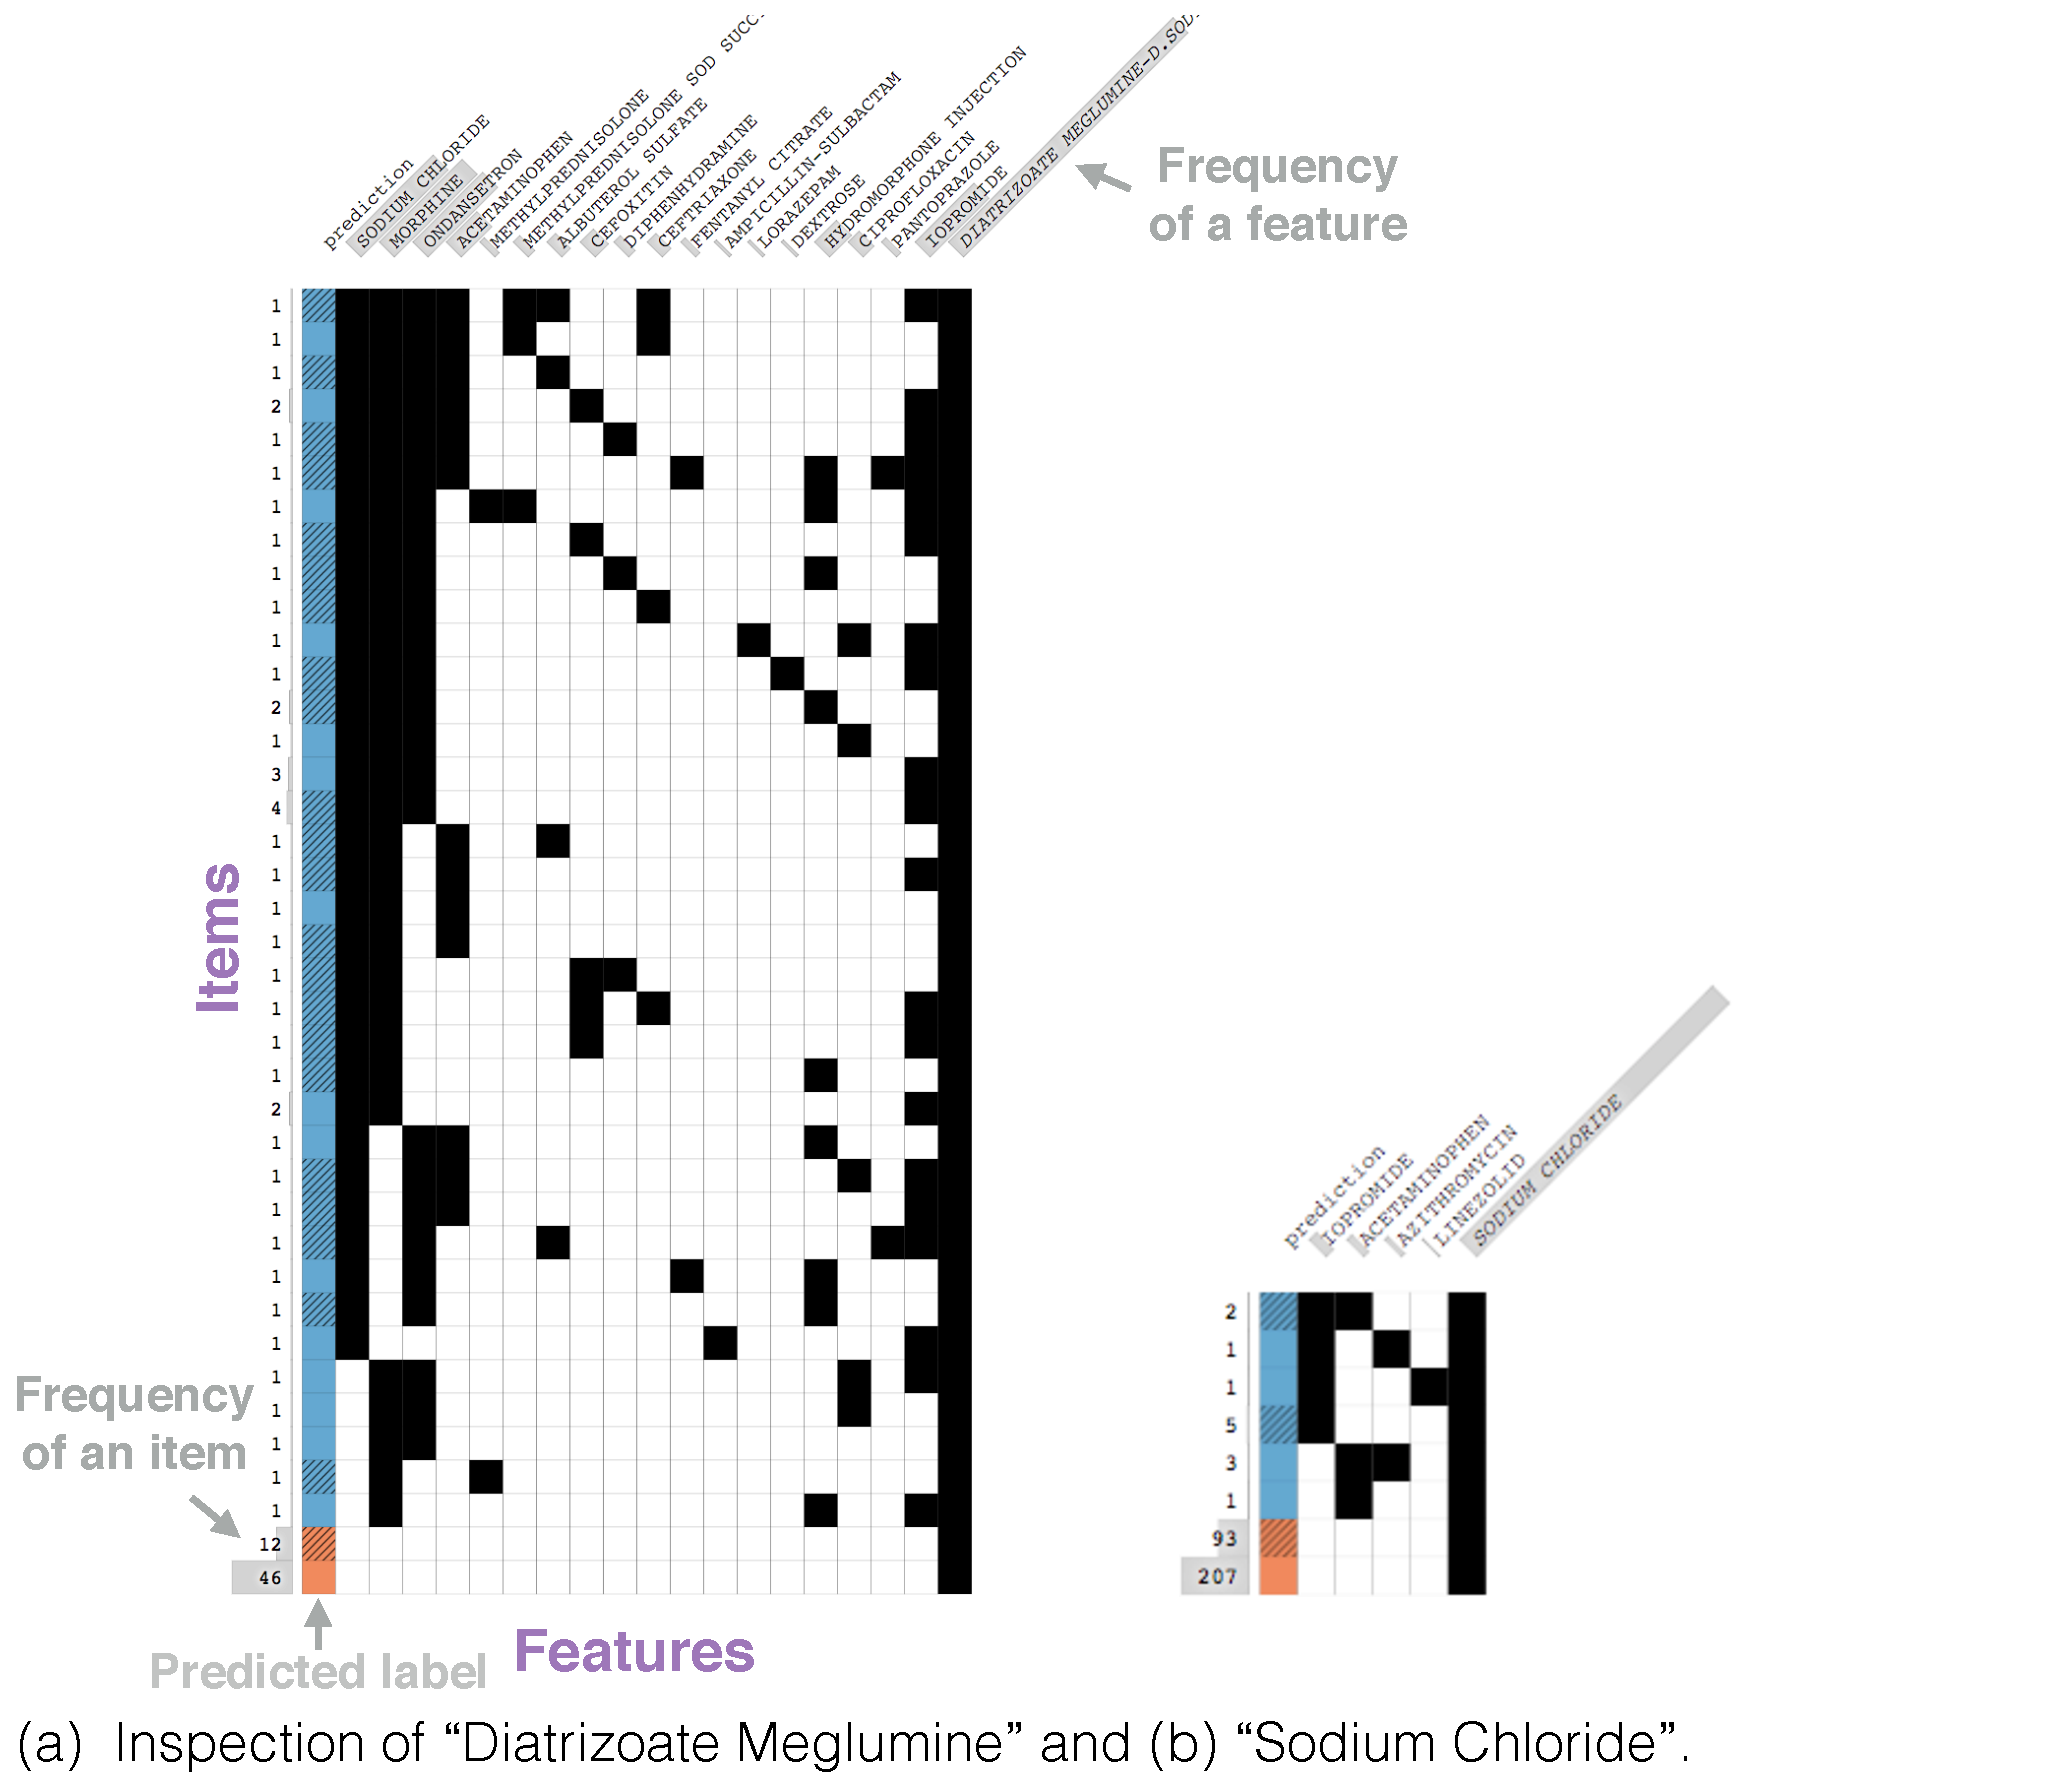
\includegraphics[width=\linewidth]{explainer/inspect1}
% \begin{subfigure}[b]{0.7\linewidth}
%     \centering
%     \includegraphics[width=\linewidth]{fig/inspect}
%     \caption{~Inspection of ``Diatrizoate Meglumine"}
%     \label{figs:inspect}
% \end{subfigure}
% \hspace{-3em}
% \begin{subfigure}[b]{0.35\linewidth}
%     \centering
%     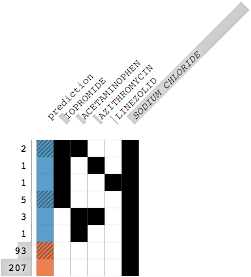
\includegraphics[width=1.03\linewidth]{fig/sodchl} % warning here is necessary
%     \caption{~and ``Sodium Chloride".}
%     \label{figs:sodchl}
% \end{subfigure}
\caption[The \tabC.]{
The \textbf{\tabC} showing a matrix of data items as rows and features as columns for the explanations \emph{Diatrizoate Meglumine} and \emph{Sodium Chloride} in the initial data set of the case study (Section~\ref{sec:case_study}).
Rows group identical instances together and show the count on the left side.
Features are sorted by ``relative feature importance" showing from left to right how labels can be separated.
% \aritra{This figure needs annotations: Items, Features, Predicted Label, and what the bars mean}
% \joschi{too much info here}
}
\label{figs:inspect_all}
\end{figure}

Another common explanation is \emph{Ibuprofen} a pain relieving drug.
It is predictive for non-admissions which is likely due to patients with pain symptoms that turned out to be benign.
The odds ratio indicates a significant relation to the outcome.
On the other hand \emph{Vancomycin}, an antibiotic used for treating infections, is significantly linked to hospital admission which is expected.

After filtering out uncommon explanations ($< 20$ explained items) ordering the explanations by ``odds ratio" reveals significant indicators for admission and non-admission (Figure~\ref{figs:expl_10_or_pos}).
In addition to the already discovered significant explanations we can see \emph{Furosemide}, a drug for treating congestive heart failure, as being strongly indicative for admission and certain drugs in combination with \emph{Sodium Chloride} strongly linked to non-admission (Figure~\ref{figs:expl_10_or_neg}).
The drugs in question are pain-relievers (\emph{Morphine} and \emph{Ketorolac}) and drugs to help with stomach problems (\emph{Ondansetron} and \emph{Metoclopramide}).
Note that using an IV (\emph{Sodium Chloride}) for stomach related problems helps both hydrate the patient and ensures the intake of the medication (after \eg, vomiting).

% 0:17:40;00
\par \noindent \textbf{Finding Weaknesses (G4).}
Ordering explanations by ``uncertainty" (Figure~\ref{figs:expl_10_uncertain}) shows explanations whose predictions are not significant.
This is often the case when it is impossible to correctly predict a set of identical instances that have a contradicting ground truth.

The first two explanations \emph{Ipratropium Bromide}, \emph{Albuterol Sulfate} (medication for treating chronic obstructive pulmonary disease and asthma, lung diseases that can have chronic and acute symptoms the latter of which requires immediate attention) and \emph{Sodium Chloride}, \emph{Ondansetron}, \emph{Morphine} are both predicted negative.
However, the ground truth of those subset has the same distribution as the overall dataset (thus an odds ratio close to 1).
This means the true admission rate of those two subsets is independent of the medication in question as the admission rate matches the admission rate of the dataset.
If more patients would be observed in the data this rate would likely stay the same.
Through \tabC we can see that the features of the explanations are the only features in the respective data items.
No further information is provided that could help swaying those subsets in a definite direction of admission or non-admission.

% ``Aspirin", a blood thinner, is the most severe example as roughly $50\%$ of the items are misclassified thus switching the predicted outcome would not result in a better classification.
% In fact inspecting the data items closer using the \tabC shows that $66$ of the $131$ are feature vectors with only ``Aspirin" while their ground truth label is distributed $25$ admission to $41$ non-admission.
% Without further knowledge it is impossible to correctly classify those data items as the labels for the same feature vectors are contradictory.
% This likely stems from the fact that ``Aspirin" is given to alleviate a wide range of symptoms with diverse severeness.
% Interestingly, the odds ratio indicates a significant positive tendency as we have observed more non-admission patients overall and should thus expect an error rate closer to the admission rate if ``Aspirin" truly does not carry predictive power.

% 0:18:46;00 also talking about Iohexol (which is not in use anymore) --> marker of age / multiple hospitalizations
Another problematic drug is \emph{Diatrizoate Meglumine} which has a high misclassification rate and an odds ratio close to 1.
The drug is a contrast medium that is given in preparation of PET (positron emission tomography) or CT (computerized tomography) scans.
As the outcome of the scan is not known it cannot be determined whether the test was positive for the hypothesis made by the attending physician.
Furthermore, even the presence of other drugs is no indicator for admission as it only shows the doctor's risk assessment \textit{before} the test was ordered and therefore does not include whether the doctor's assumption was correct.
Note, that Figure~\ref{figs:inspect_all}a shows how outcomes can be better separated using available features.
However, doing so would result in overfitting on the validation data set which should be avoided in any case.

Faced with this revelation we explored how we could provide more information to reduce those ambiguities.
In order to properly deal with cases like \emph{Ipratropium Bromide} and \emph{Albuterol Sulfate} or \emph{Sodium Chloride} and \emph{Diatrizoate Meglumine} more information is needed.
Through domain expertise we can reason about the underlying shortcomings of the current dataset, \eg, the nature of the limitations of \emph{Diatrizoate Meglumin}.
In order to overcome those limitations we need to include additional information in our dataset.
For example, including information about the final diagnosis of a patient resolves the ambiguities of patients explained by \emph{Diatrizoate Meglumin} and other problematic explanations mentioned above, and likely improves the overall quality of the prediction\footnote{Including other information, such as, mode of arrival, gender, or age, might improve accuracy but would not solve the issues mentioned above.}.
However, this also moves the time of the prediction closer to the point in time when the actual decision, whether the patient is admitted to the hospital, is made thus reducing the time-gain for preparing a bed in case of admission.
% or making it not being a prediction anymore

\par \noindent \textbf{Changing Data and Model.}
In the following we describe how we could improve the prediction task by including additional information to our dataset. This additional information, \ie final diagnoses, was added to overcome limitations posed by medications not strongly linked to an outcome, as described above.
In order to include those diagnosis features in the data we had to capture new data which also allowed for capturing a bigger dataset.
The new dataset contains 154580 patients  ($20\%$ admitted) and was randomly split into a training (30916 patients with $20\%$ admitted) and test (123664 patients with $20\%$ admitted) dataset.
It contains 1709 unique medications and 15422 unique diagnoses.

The best results of different models on the new dataset are:

\begin{center}
\begin{tabular}{l|rr|rr}
\multicolumn{1}{c}{} & \multicolumn{2}{c}{no diagnoses} & \multicolumn{2}{c}{incl. diagnoses}\\
Model & Training & Test AUC & Training & Test AUC\\
\hline
GNB & 0.51 & 0.49 & 0.75 & 0.66 \\
LR & 0.71 & 0.67 & 0.93 & 0.88 \\
RF & 0.69 & 0.68 & 0.98 & 0.83 \\
MLP & 0.71 & \textbf{0.68} & 0.95 & \textbf{0.88} \\
\multicolumn{5}{c}{{\scriptsize Maximum values are chosen using digits not shown.}} \\
\end{tabular}
\end{center}

Again we are focusing solely on the Multi Layer Perceptron model for further analyses (even though similar results can be found with the other equally well performing models).
In order to compare our new data to the previous dataset we first created models that do not utilize the newly added diagnoses.
However, the resulting AUC is much lower than for the initial data.
Looking at the \tabA reveals a strong concentration of data points at a specific prediction score.
% 0:03:00;00
Focusing on this prediction score in the \tabB (Figure~\ref{figs:adm_10_size}) shows that it corresponds to the 62776 patients that did not receive any medication at all.
This configuration predicts non-admission as it is more likely to get sent home when not receiving any medication.
The unusual large number of such cases ($\sim\hspace{-0.2em}50\%$), however, hints at a possible capturing error which would also explain the 11394 cases where patients were admitted.
This failure rate severely affects the machine learning models.
For comparison the next largest explanation of \emph{Ibuprofen} in the new dataset consists only of 2011 patients.
In fact patients without medication were not captured in the original dataset and removing them from the new dataset increases the best train / test AUC to $0.83$ / $0.80$ similar to the original dataset.
For further analysis we include patients without medication.
Utilizing diagnoses in the models strongly increase the possible AUC.

\par \noindent \textbf{How Did Diagnoses Features Change the Model?}
The \tabB of the best model utilizing diagnoses features, Multi Layer Perceptron, can be seen in Figure~\ref{figs:adm_10_diag}.
Noticeably, almost all explanations now consist of diagnoses.
This also means that medication features have now become almost irrelevant except for medications, like \emph{Ibuprofen} and \emph{Vancomycin}, that were strong indicators before.
The most significant diagnoses, using odds ratio, for admission are \emph{Sepsis}, \emph{Sepsis due to unidentified organism}, and \emph{Small Bowel Obstruction}.
Diagnoses that require antibiotics (\eg, \emph{Vancomycin}) and pain medication (\eg, \emph{Ibuprofen}) respectively.
Contradictory or insignificant medications, like \emph{Diatrizoate Meglumine} or \emph{Ipratropium Bromide} and \emph{Albuterol Sulfate}, do not show up anymore as they can be more effectively replaced by their diagnoses.
% 0:00:00;00
The largest explanation, with 2619 patients, is \emph{Unspecified} which, after some research, turns out to be due to a policy change before which doctors were allowed to omit a diagnosis if the patient got admitted to the hospital.
Why only 2105 ($\sim\hspace{-0.2em}80\%$) were actually admitted to the hospital remains unclear.

\begin{figure}
\centering
\begin{subfigure}[b]{0.75\linewidth}
    \hfill
    \includegraphics[height=7em]{explainer/adm_10_size}
    \caption{~The second dataset without diagnoses ordered by ``total" size.}
    \label{figs:adm_10_size}
\end{subfigure}
\\
\begin{subfigure}[b]{0.75\linewidth}
    \hfill
    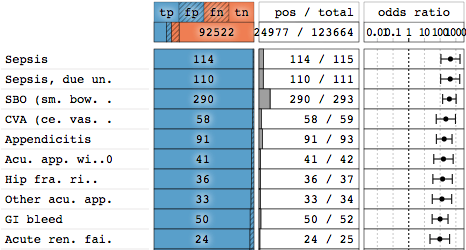
\includegraphics[height=7em]{explainer/adm_10_or_full}
    \caption{~The second dataset using diagnoses ordered by ``odds ratio".}
    \label{figs:adm_10_diag}
\end{subfigure}%
\caption[Showing the second dataset of the case study.]{Showing the second dataset of the case study (Section~\ref{sec:case_study}) with and without using diagnoses features in the \textbf{\tabB}.}
\end{figure}
% \begin{figure}
% \centering
% \begin{subfigure}[b]{\linewidth}
%     \hfill
%     \includegraphics[height=9.5em]{fig/adm_10_size}
%     \caption{~The second dataset without diagnoses ordered by ``explanation length".}
%     \label{figs:adm_10_size}
% \end{subfigure}
% \\
% \begin{subfigure}[b]{1.01\linewidth}
%     \hfill
%     \includegraphics[height=9.5em]{fig/adm_10_diag}
%     \caption{~The second dataset (filtered by $total > 200$) using diagnoses ordered by ``odds ratio".}
%     \label{figs:adm_10_diag}
% \end{subfigure}%
% \\
% \begin{subfigure}[b]{\linewidth}
%     \hfill
%     \includegraphics[height=9.5em]{fig/adm_10_or_nodiag}
%     \caption{~The second dataset (filtered by $total > 200$) without diagnoses ordered by ``odds ratio".}
%     \label{figs:adm_10_or_nodiag}
% \end{subfigure}%
% \\
% \begin{subfigure}[b]{\linewidth}
%     \hfill
%     \includegraphics[height=9.5em]{fig/adm_10_or_ff}
%     \caption{~The first biased dataset (filtered by $total > 200$) ordered by ``odds ratio".}
%     \label{figs:adm_10_or_ff}
% \end{subfigure}
% \\
% \begin{subfigure}[b]{\linewidth}
%     \hfill
%     \includegraphics[height=16em]{fig/adm_ft}
%     \caption{~The second biased dataset ordered by ``incorrect".}
%     \label{figs:adm_ft}
% \end{subfigure}
% \caption{Datasets as they are discussed in Section~\ref{sec:case_study} and Section~\ref{sec:bias}.}
% \end{figure}

\par \noindent \textbf{Diagnostic Insights.}
By adding diagnoses to the dataset a strong increase in predictive quality was achieved.
However, seeing that diagnoses effectively replace medication in their predictive power suggests that the ``labels are leaking".
That is, since doctors make the decision of whether to admit a patient at the time of the final diagnosis there is a strong correlation between the label and the features.
This is an undesired effect as the model is not predicting the outcome anymore but merely building an approximate lookup table for diagnosis admission rates.
If the model would have kept using medication and only consulted diagnoses for ambiguous cases the usability of the model would have been improved due to diagnoses.
This is not the case.
Despite its lower objective quality the model using only medications as input emerged as the more practically useful model.
Since experts know about the strengths and weaknesses of the model, they can distinguish between confident and ambiguous cases early and decide whether to accept the prediction or wait for the final decision made by the doctor.
This demonstrates that a statistically weaker model can be more useful in practice.

% \section{Data Bias Detection}
% \label{sec:bias}
% In addition to the case study we derived synthetic datasets in order to test if certain data biases can be detected using our workflow and what the limitations of those are.
% For this we created two artificial datasets showing systematic biases.
% The first dataset contains a systematic bias in both the training and the test data.
% The second dataset on the other hand contains this bias only in the training data.

% For the synthetic datasets we used the case study data with observed diagnoses.
% We used only the medication for training the model while we utilized the diagnoses to create biases in the data.
% For our experiments we altered patients with the word ``alcohol" in the diagnosis.
% In the original dataset of 154580 patients in total 4577 have an alcohol related diagnosis and of those only 405 got admitted to the hospital.
% Typically, patients with these diagnoses are put under observation which counts as non-admission in our labels.

% In the first scenario we changed the labels of those 4577 patients to hospital admission.
% This simulates the case where the entire data is biased.
% For example, such a situation could occur if a hospital uses non-standard procedures.
% Using the ``odds ratio" order in the \tabB (see Figure~\ref{figs:adm_10_or_ff}) the most significant explanation now is ``Folic Acid" and ``Chlordiazepoxide".
% Both medications are typically used to alleviate alcohol withdrawal symptoms.
% Those medications did not show up remarkably before and if so are expected to show up in a context of non-admission (see Figure~\ref{figs:adm_10_or_nodiag}).
% Thus seeing those medications in this context immediately raises suspicion in doctors.

% In the second scenario we only changed the labels of those patients in the \textit{training} set to hospital admission.
% The test set remains unchanged.
% This simulates the case where the model is trained in an environment with a different bias than where it is applied.
% For example, such a situation could occur when a model is trained using data from one hospital and is implemented in another hospital.
% In our simulated data, using the ``incorrect" predictions order in the \tabB (see Figure~\ref{figs:adm_ft}), we get high error rate explanations containing ``Folic Acid", ``Chlordiazepoxide", and ``Thiamine".
% ``Thiamine" is given to counter alcohol induced thiamine shortage.
% Those explanations have a high misprediction rate as they were trained with a dataset that has a different ground truth than the test dataset in those cases.

% As we can see with those scenarios our method can detect errors that occur from which data items a model regards as being similar.
% The technique is limited by errors that occur because the model did not see relevant examples during training.
% In such cases data items get explained differently.
% However, this does not imply that this other explanation is not also a correct one.

% Another limitation of explanations is the detection of similar behaving features.
% If a feature $A$ and a feature $B$ behave similarly but never occur together they will show up as two different explanations despite them likely being merged in the model.
% This makes features seem less prominent in case, for example, there exist multiple names for the same medication.
% In order to solve this limitation it is thinkable to utilize model internal information to retrieve which features are merged and treated the same within the model.
